\documentclass[aspectratio=169]{beamer}
\usetheme{Boadilla}
%\usetheme{Warsaw}
%\setbeamercovered{transparent}
\beamertemplatetransparentcoveredhigh
\usepackage[portuges]{babel}
\usepackage[utf8]{inputenc}
\usepackage{lmodern}
\usepackage[T1]{fontenc}
\usepackage{hyperref} 


\newcommand{\eng}[1]{\textsl{#1}}
\newcommand{\cod}[1]{\texttt{#1}}

\title[Apresentação da Disciplina]{Algoritmo e Estrutura de Dados II}
\subtitle{Apresentação da Disciplina}
\author[Frederico Santos de Oliveira]{prof. Frederico Santos de Oliveira}
\institute[UFMT]{Universidade Federal de Mato Grosso\\ Faculdade de Engenharia}
\date{}

\begin{document}

\begin{frame}[plain]
  \titlepage
\end{frame}

%\section*{Roteiro}

\begin{frame}
  \frametitle{Agenda}
  \tableofcontents
\end{frame}

\section{Introdução}

\begin{frame}{Quem sou Eu}
\begin{columns}[T] % align columns
\begin{column}{.30\textwidth}
{\bf Frederico S. Oliveira}
\begin{figure}[h]
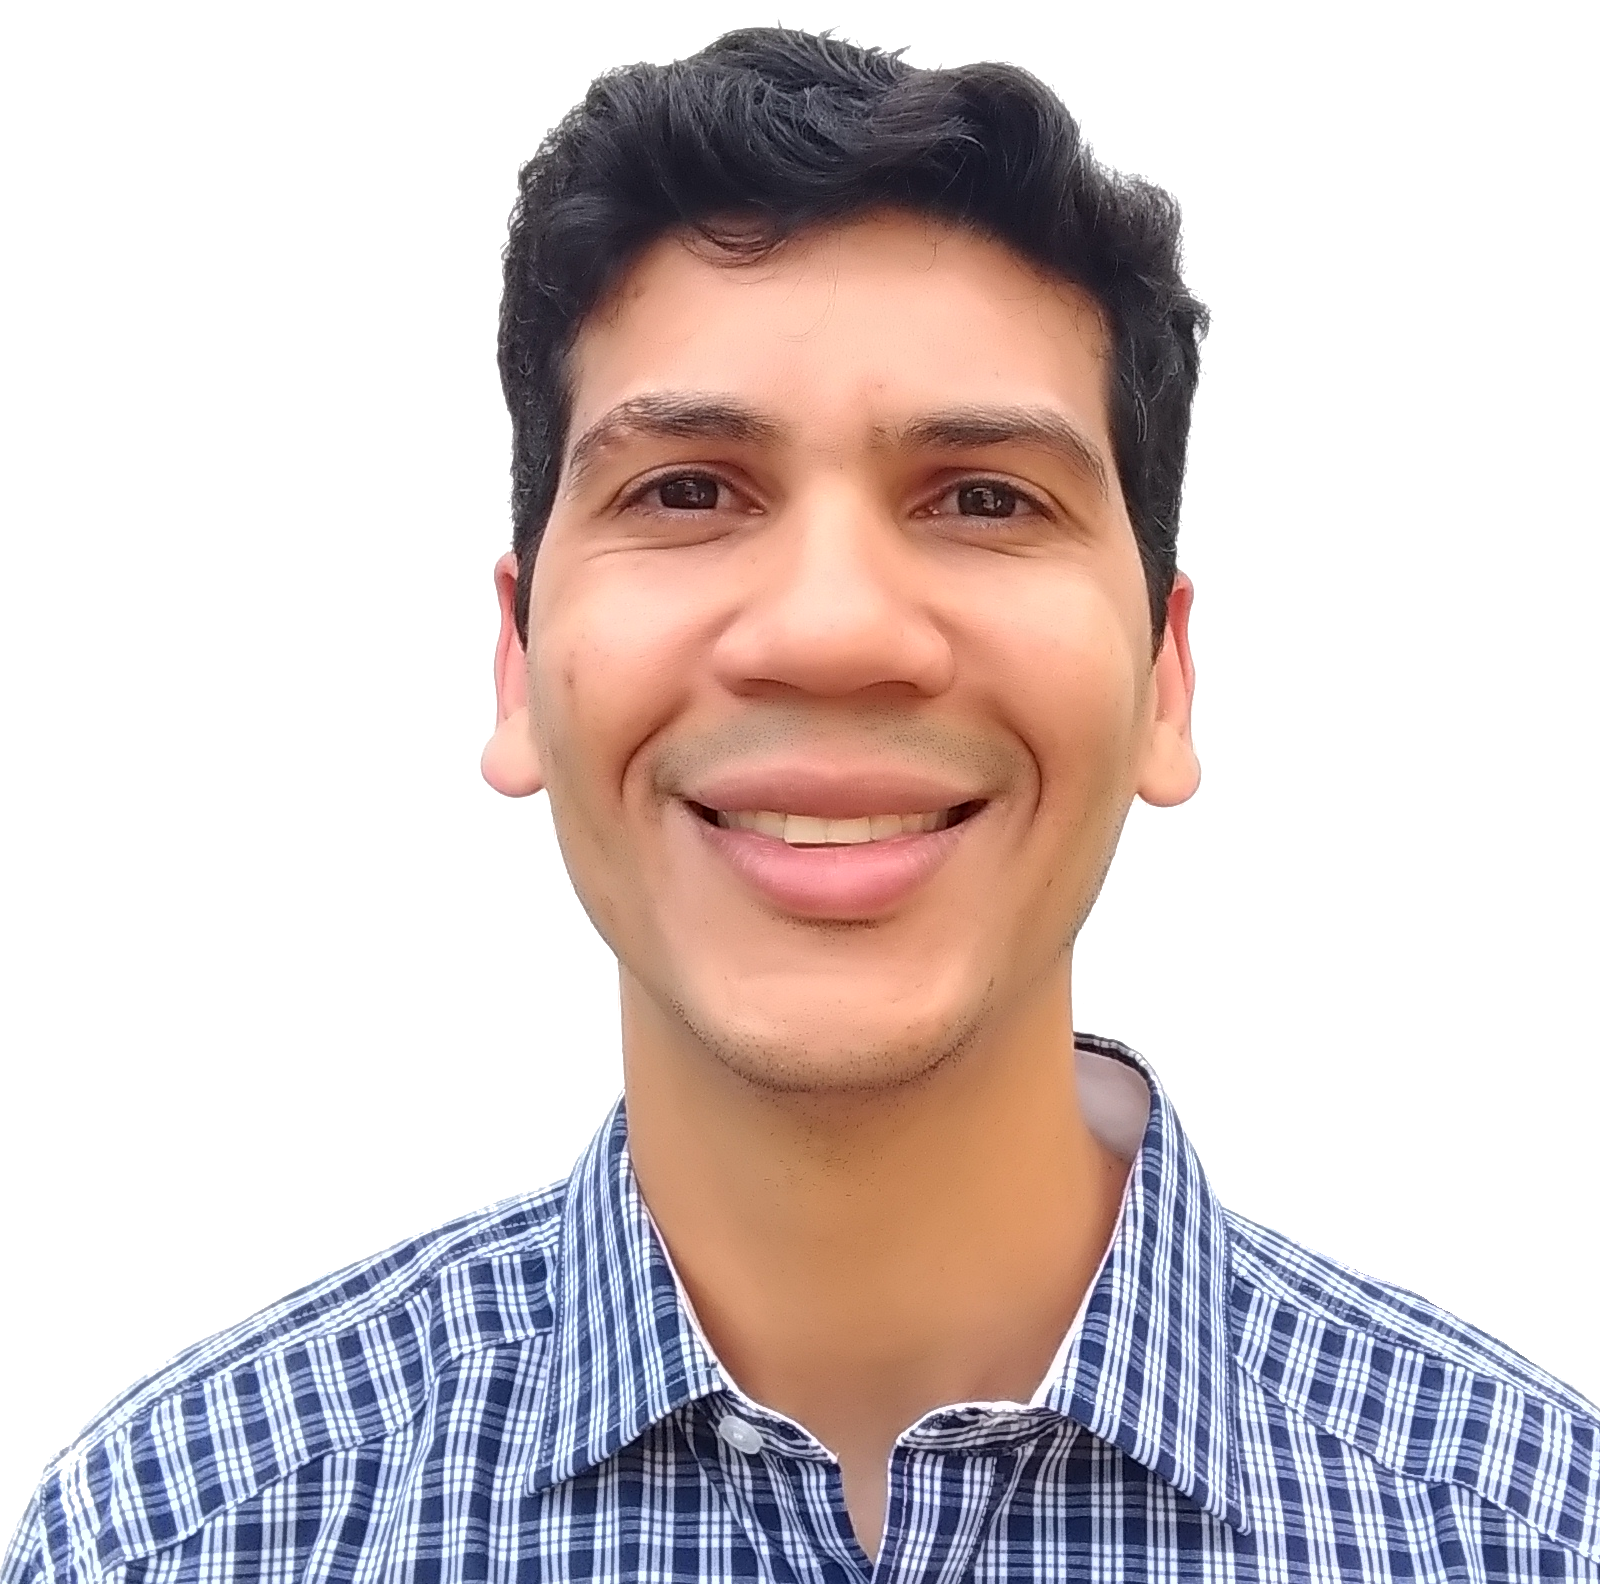
\includegraphics[width=3.5cm]{imgs/perfil.png}
\end{figure}
\end{column}%
\hfill%
\begin{column}{.64\textwidth}
\begin{itemize}
\item Bacharel e Mestre em Ciência da Computação (UFLA). 
\item Doutorando em Inteligência Artificial (UFG). 
\item Professor UFMT:
\begin{itemize}
\item Agoritmos e Estrutura de Dados I
\item Agoritmos e Estrutura de Dados II
\item Agoritmos e Estrutura de Dados III
\item Inteligência Artificial
\end{itemize}
\item \href{http://freds0.github.io}{http://freds0.github.io}
\item fred.santos.oliveira@gmail.com
\end{itemize}
\end{column}%

\end{columns}
\end{frame}

\section{Ementa da disciplina}

\begin{frame}
\frametitle{Ementa da disciplina}
\begin{itemize}
\item Revisão: ponteiros e estruturas de dados.
\item Análise de algoritmos.
\item Algoritmos de Ordenação.
\item Pilhas, filas e Listas. 
\end{itemize}
\end{frame}

\begin{frame}
\frametitle{Objetivo Geral}
\begin{itemize}
 \item Apresentar as principais estruturas de dados e mostrar suas aplicações em problemas.
\end{itemize}
\end{frame}

\begin{frame}
\frametitle{Objetivos Específicos}
\begin{itemize}
 \item Os trabalhos serão desenvolvidos utilizando a linguagem C.
 \item No entanto, esta disciplina \underline{não} é um curso de C.
 \item Portanto, os algoritmos são apresentados utilizando pseudo-código.
 \item Para aqueles não familiarizados com a linguagem C, recomenda-se o estudo utilizando o livro C - Como programar. 
 %\item Dúvidas sobre a linguagem podem ser resolvidas nas aulas práticas ou com os monitores da disciplina.
\end{itemize}
\end{frame}


\section{Conteúdo Programático}

\begin{frame}
\frametitle{Conteúdo Programático}
Unidade I - Alocação de Memória
\begin{itemize}
 \item Ponteiros
 \item Organização da Memória
 \item Manipulação da Memória
 \item Ponteiros Duplos
\end{itemize}
\end{frame}

\begin{frame}
\frametitle{Conteúdo Programático}
Unidade II - Tipos Abstratos de Dados
\begin{itemize}
 \item Registros (struct)
 \item Declaração de Tipos (typedef)
 \item Atribuições
 \item Tipos Abstratos de Dados
\end{itemize}
\end{frame}


\begin{frame}
\frametitle{Conteúdo Programático}
Unidade III - Análise Assintótica
\begin{itemize}
 \item Tempo de Processamento
 \item Comportamento Assintótico
 \item Análise Pior Caso
 \item Análise Caso Médio
 \item Análise Melhor Caso
\end{itemize}
\end{frame}

\begin{frame}
\frametitle{Conteúdo Programático}
Unidade IV - Algoritmos de Ordenação
\begin{itemize}
 \item Bubblesort
 \item Selectionsort
 \item Insertionsort
 \item Shellsort
 \item Mergesort
 \item Heapsort
 \item Quicksort
 \item Countingsort
\end{itemize}
\end{frame}


\begin{frame}
\frametitle{Conteúdo Programático}
Unidade V - Busca Binária
\begin{itemize}
 \item Pesquisa Sequencial
 \item Pesquisa Binária
\end{itemize}
\end{frame}

\begin{frame}
\frametitle{Conteúdo Programático}
Unidade VI - Estrutura de Dados
\begin{itemize}
 \item Lista, fila e pilha utilizando alocação estática
 \item Lista, fila e pilha utilizando alocação dinâmica
\end{itemize}
\end{frame}

\section{Metodologia}

\begin{frame}
\frametitle{Metodologia}
Metodologia
\begin{itemize}
 \item Vídeo-Aulas assíncronas disponibilizadas on-line
 \item Aulas síncronas para esclarecimento de dúvidas.
 \item Desenvolvimento de exercícios.
 \item Uso do Ambiente Virtual de Aprendizagem (www.ava.ufmt.br)
 \item Uso do sistema de submissão de trabalhos (www.run.codes)
\end{itemize}
\end{frame}

\section{Avaliações}

\begin{frame}
\frametitle{Avaliações}
Três Avaliações Práticas 
\begin{itemize}
 \item T1 (33\%)
 \item T2 (33\%)
 \item T3 (34\%) 
\end{itemize}
\end{frame}


\begin{frame}
\frametitle{Avaliações}
 A Média Final (MF) das avaliações será calculada pela fórmula: 
 \begin{eqnarray}
   MF &=& (T1 + T2 + T3) / 3 \nonumber
 \end{eqnarray}
\end{frame}

\begin{frame}
\frametitle{Avaliações}
A situação $S(MF)$ do aluno, em que $MF$ é a Média Final, é definida pela equação:
\begin{equation}
\label{fib}
  S(MF)=
  \left\{
   \begin{array}{ll}
    Aprovado & \mbox{se\ }MF\geq 50 \\
    Reprovado & \mbox{caso contrário};\
   \end{array}
  \right.\nonumber
\end{equation}
\end{frame}

%
%\begin{frame}
%\frametitle{Avaliações}
%Avaliações
%\begin{itemize}
% \item Faltas acima de 25\% da carga horária implicarão em reprovação.
% \item Ou seja, faltas acima de $0.25 \times 96 = 24$ horas-aula implicarão em reprovação. 
% \item Cada dia de aula conta como duas horas-aula. Portanto, faltas acima de 12 (doze) dias de aula implicarão em reprovação.  
%\end{itemize}
%\end{frame}

\section{Bibliografia}

\begin{frame}
\frametitle{Bibliografia Utilizada}
\begin{itemize}
 \item ZIVIANI, N. Projeto de Algoritmos: com implementações em Pascal e C.
Cengage Learning, 2010.
 \item CORMEN, T. H. Algoritmos - Teoria e Prática. Elsevier, 2009.
 \item DEITEL, H. C - Como programar. Pearson, 2011.
 \item SEDGEWICK, R. Algorithms. 4th ed. Addison-Wesley, 2011.
\end{itemize}
\end{frame}


\begin{frame}
  \frametitle{FIM}
\centering
\huge{Dúvidas?}
\end{frame}	


\end{document}
